\usetikzlibrary{arrows.meta}
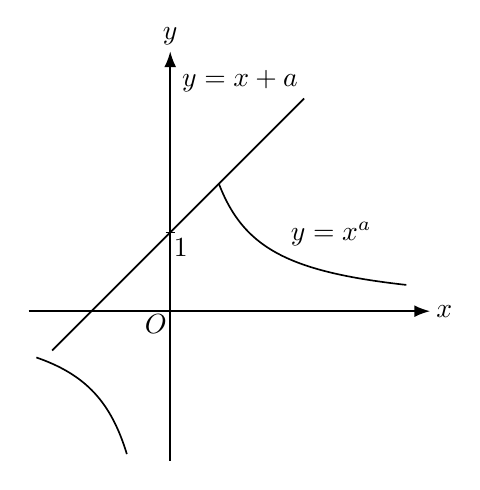
\begin{tikzpicture}[x=1cm,y=1cm,line width=.6pt,>=Latex,font=\normalsize]
\draw[->] (-1.8,0)--(3.3,0) node[right,inner sep=0pt,xshift=2pt] {$x$};
\draw[->] (0,-1.9)--(0,3.3) node[above,inner sep=0pt,yshift=2pt] {$y$};
\draw[domain=-1.5:1.7,samples=2] plot (\x,{\x+1});
\draw[domain=0.618034:3.0,samples=161] plot (\x,{1/\x});
\draw[domain=-1.7:-0.55,samples=101] plot (\x,{1/\x});
\node[above left,inner sep=2pt] at (1.7,2.7) {$y=x+a$};
\node[above right,inner sep=2pt] at (1.45,0.75) {$y=x^a$};
\draw (-0.06,1)--(0.06,1);
\node[below right,inner sep=0pt,xshift=1pt,yshift=-1pt] at (0,0.97) {$1$};
\node[below left,inner sep=1pt] at (0,0) {$O$};
\end{tikzpicture}
